%------------------------------------------------
%----------------------------------------------------------------------------------------
\section{DWARF}
%----------------------------------------------------------------------------------------
%------------------------------------------------
%------------------------------------------------
\begin{frame}{How dose debuggers work?}
	\begin{figure}
		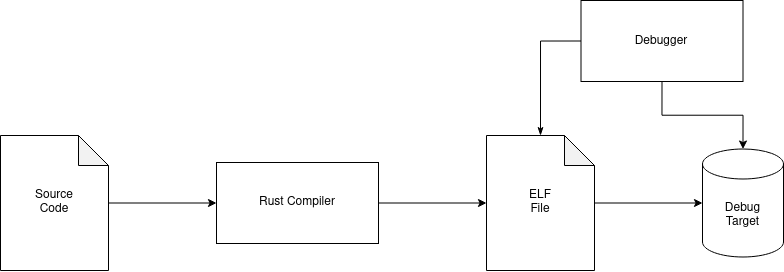
\includegraphics[width=0.7\textwidth,height=0.40\textwidth,keepaspectratio]{gen_debug_info.png}
	\end{figure}
\end{frame}

%------------------------------------------------
%------------------------------------------------
\begin{frame}{DWARF}
	\begin{figure}
		
\includegraphics[width=0.9\textwidth,height=0.48\textwidth,keepaspectratio]{gimli.jpeg}
	\end{figure}
\end{frame}

%------------------------------------------------
%------------------------------------------------

\begin{frame}{DWARF}
	\begin{figure}
		
\includegraphics[width=0.3\textwidth,height=0.48\textwidth,keepaspectratio]{dwarf_logo.png}
	\end{figure}
\end{frame}

%------------------------------------------------
%------------------------------------------------
\begin{frame}{How to get the debug information?}
    \begin{itemize}
	    \item DWARF is used to understand how the source and machine code relates to each other.
	    \item ELF contains the Debugging with Attributed Record Formats(DWARF).
	    \item Rust uses DWARF version 4.
	    \item Dwarf is divided into 12 sections.
    \end{itemize}
\end{frame}

%------------------------------------------------
%------------------------------------------------

\begin{frame}{DWARF Sections}
	\begin{figure}
		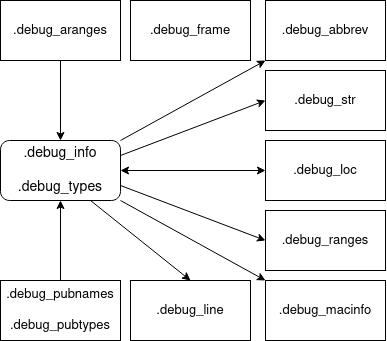
\includegraphics[width=0.9\textwidth,height=0.40\textwidth,keepaspectratio]{dwarf-sections.png}
	\end{figure}
\end{frame}

%------------------------------------------------
%------------------------------------------------

\begin{frame}{Compilation unit}


    \begin{columns}[c] % The "c" option specifies centered vertical alignment while the "t" option is used for top vertical alignment

        \column{.45\textwidth} % Left column and width
        \begin{itemize}
		\item Sections .debug\_info and .debug\_types contain a number of compilation units.
		\item A compilation unit can be a program or a library.
		\item Each compilation unit contains all the related debug information for that unit.
		\item Each compilation unit contains a tree of DIEs.
        \end{itemize}

        \column{.5\textwidth} % Right column and width
	\begin{figure}
		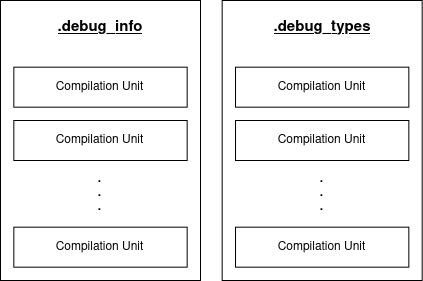
\includegraphics[width=1\textwidth,height=0.50\textwidth,keepaspectratio]{compilation_unit.png}
	\end{figure}

    \end{columns}
\end{frame}

%------------------------------------------------
%------------------------------------------------

%\begin{frame}{Compilation unit}
%	\begin{figure}
%		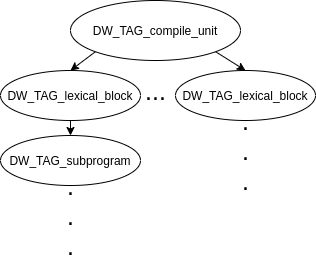
\includegraphics[width=0.9\textwidth,height=0.40\textwidth,keepaspectratio]{die-tree.png}
%	\end{figure}
%\end{frame}

%------------------------------------------------
%------------------------------------------------

\begin{frame}{Debug Information Entry(DIE)}
	\begin{itemize}
	    \item Debug Information Entry(DIE).
		\begin{itemize}
	    		\item All DIEs have a DWARF TAG.
	    		\item DIEs also contain a number of DWARF attributes.
		\end{itemize}
	    \item DWARF DIE example from the .debug\_info section.
	\end{itemize}
	\begin{figure}
		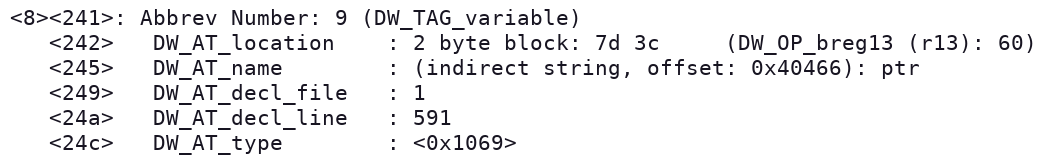
\includegraphics[width=0.9\textwidth,height=0.48\textwidth,keepaspectratio]{dwarf-die.png}
	\end{figure}
\end{frame}

%------------------------------------------------
%------------------------------------------------

\begin{frame}{An example on how to use DWARF}
	\begin{itemize}
	    \item How can DWARF be used to evaluate the value of a variable?
		\begin{itemize}
		    \item Two things are needed from DWARF.
			\begin{itemize}
			    \item Location of the value in the debug target.
			    \item The type of the variable.
			\end{itemize}
		\end{itemize}
	\end{itemize}
\end{frame}

%------------------------------------------------
%------------------------------------------------

\begin{frame}{Evaluating a variable}
	\textbf{Finding the relevant debug information}
	\begin{enumerate}
		\item Read the current code location from the debug target.
		\item Find the current compilation unit using the current code location.
		\item Find the current subprogram DIE using the current code location.
		\item Find the searched variable DIE in the sub tree of the subprogram DIE. 
	\end{enumerate}
\end{frame}

%------------------------------------------------
%------------------------------------------------

\begin{frame}{Evaluating the location of a variable}
	\begin{figure}
		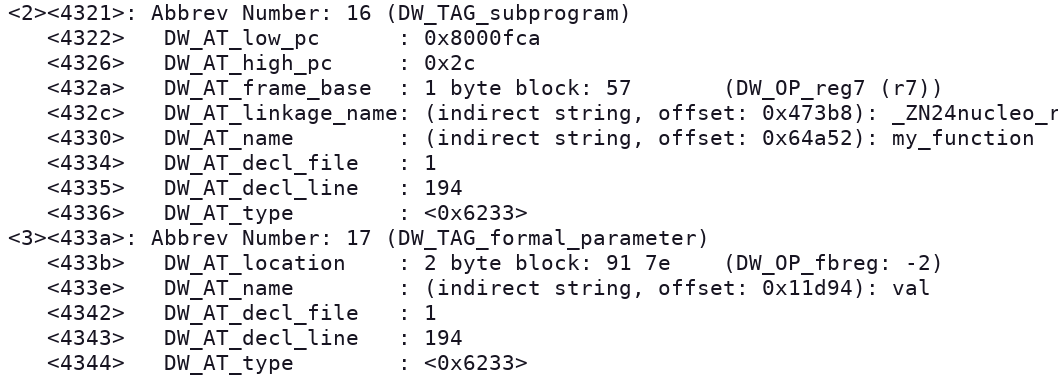
\includegraphics[width=0.9\textwidth,height=0.48\textwidth,keepaspectratio]{subprogram-example.png}
	\end{figure}
\end{frame}

%------------------------------------------------
%------------------------------------------------

\begin{frame}{Parsing the type of a variable}
	\begin{figure}
		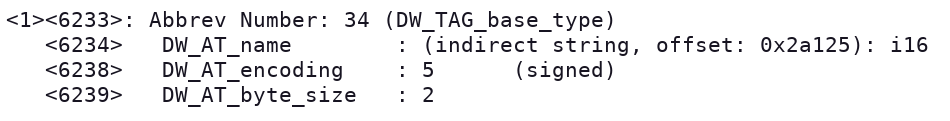
\includegraphics[width=0.9\textwidth,height=0.48\textwidth,keepaspectratio]{basetype-example.png}
	\end{figure}
\end{frame}

%------------------------------------------------


%%------------------------------------------------
%\begin{frame}{DWARF}
%	\begin{figure}
%		
\includegraphics[width=0.9\textwidth,height=0.48\textwidth,keepaspectratio]{gimli.jpeg}
%	\end{figure}
%\end{frame}
%
%%------------------------------------------------
%%------------------------------------------------
%
%\begin{frame}{DWARF}
%	\begin{figure}
%		
\includegraphics[width=0.9\textwidth,height=0.48\textwidth,keepaspectratio]{dwarf_logo.png}
%	\end{figure}
%\end{frame}
%
%%------------------------------------------------
%%------------------------------------------------
%
%\begin{frame}{DWARF}
%    \begin{itemize}
%	    \item Debugging with Attributed Record Formats(DWARF)
%	    \item Debug information format
%	    \item Rust uses DWARF version 4
%	    \item DWARF is divided into 12 sections
%	    \item Executable and Linkable Format(ELF)
%    \end{itemize}
%\end{frame}
%
%%------------------------------------------------
%%------------------------------------------------
%
%\begin{frame}{DWARF Sections}
%	\begin{figure}
%		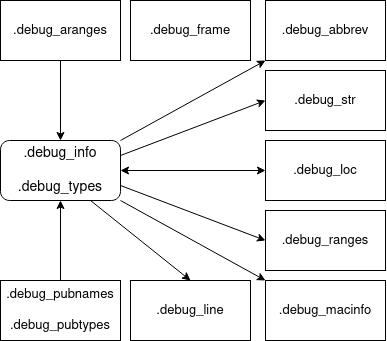
\includegraphics[width=0.9\textwidth,height=0.48\textwidth,keepaspectratio]{dwarf-sections.png}
%	\end{figure}
%\end{frame}
%
%%------------------------------------------------
%%------------------------------------------------
%
%\begin{frame}{Debug Information Entry(DIE)}
%	\begin{itemize}
%	    \item Debug Information Entry(DIE).
%	    \item DWARF Attributes.
%	    \item DWARF DIE example from the .debug\_info section.
%	\end{itemize}
%	\begin{figure}
%		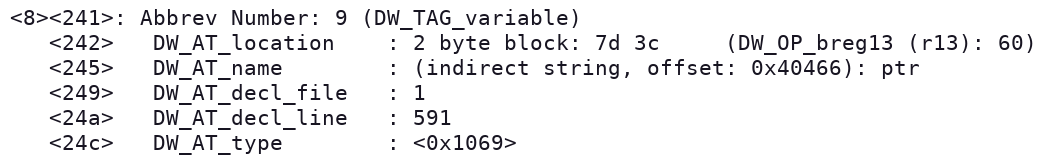
\includegraphics[width=0.9\textwidth,height=0.48\textwidth,keepaspectratio]{dwarf-die.png}
%	\end{figure}
%\end{frame}
%
%%------------------------------------------------
%%------------------------------------------------
%
%\begin{frame}{Compilation unit}
%	\begin{itemize}
%		\item Computer program is divided into compilation units.
%		\item Each compilation unit contains a DIE tree.
%	\end{itemize}
%\end{frame}
%
%%------------------------------------------------
%%------------------------------------------------
%
%\begin{frame}{Compilation unit}
%	\begin{figure}
%		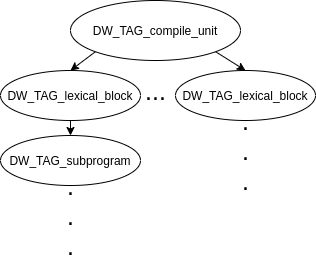
\includegraphics[width=0.9\textwidth,height=0.48\textwidth,keepaspectratio]{die-tree.png}
%	\end{figure}
%\end{frame}
%
%%------------------------------------------------
%%------------------------------------------------
%
%\begin{frame}{Evaluating a variable}
%	\begin{itemize}
%		\item Find the current compilation unit.
%		\item Find the current subprogram die.
%		\item Find the searched variable die. 
%		\item Two parts to evaluating a variable:
%			\begin{itemize}
%				\item Finding the location of the variable
%				\item Parsing the value into the correct type
%			\end{itemize}
%	\end{itemize}
%\end{frame}
%
%%------------------------------------------------
%%------------------------------------------------
%
%\begin{frame}{Evaluating the location of a variable}
%	\begin{figure}
%		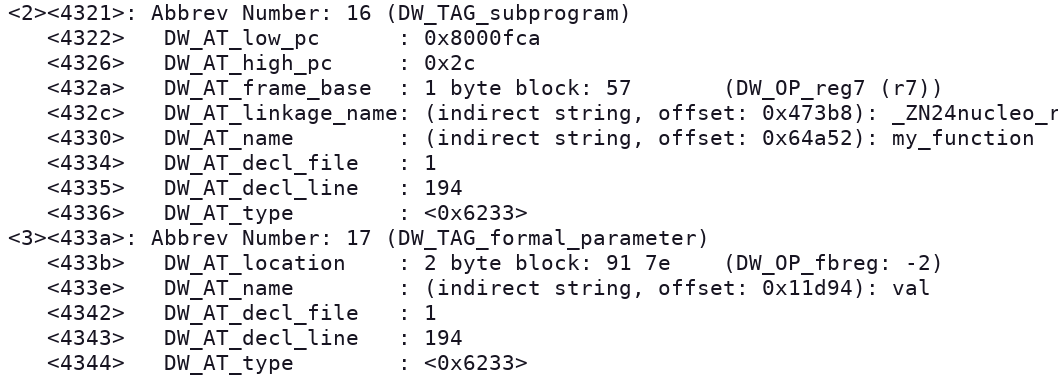
\includegraphics[width=0.9\textwidth,height=0.48\textwidth,keepaspectratio]{subprogram-example.png}
%	\end{figure}
%\end{frame}
%
%%------------------------------------------------
%%------------------------------------------------
%
%\begin{frame}{Parsing the type of a variable}
%	\begin{figure}
%		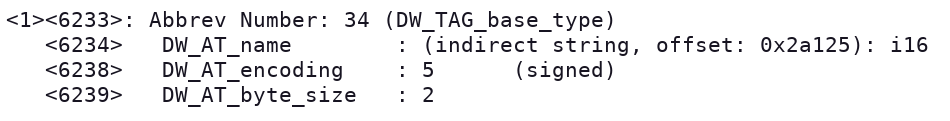
\includegraphics[width=0.9\textwidth,height=0.48\textwidth,keepaspectratio]{basetype-example.png}
%	\end{figure}
%\end{frame}
%
%%------------------------------------------------
%%------------------------------------------------
%
%\begin{frame}{Virtually Unwinding Call Stack}
%    \begin{itemize}
%        \item Stack of subroutine activation's.
%        \item A subroutine activation consists of:
%    	\begin{itemize}
%    	    \item Code location were the subroutine stopped
%    	    \item Preserved register values
%	    \item Canonical Frame Address (CFA)
%    	\end{itemize}
%        \item The needed information is in section .debug\_frame
%    \end{itemize}
%\end{frame}
%
%%------------------------------------------------
%%------------------------------------------------
%
%\begin{frame}{Virtually Unwinding Subroutine Activation's}
%    \begin{columns}[c] % The "c" option specifies centered vertical alignment while the "t" option is used for top vertical alignment
%
%        \column{.45\textwidth} % Left column and width
%        \begin{enumerate}
%        	\item Find the Common Information Entry (CIE)
%		\item Find the Frame Description Entry (FDE)
%		\item Unwind CFA and register values.
%		\item Repeat for all activation's.
%        \end{enumerate}
%
%        \column{.5\textwidth} % Right column and width
%	\begin{figure}
%		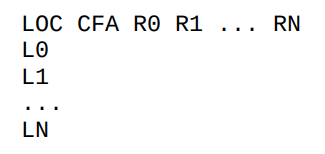
\includegraphics[width=0.9\textwidth,height=0.48\textwidth,keepaspectratio]{stacktrace-table.png}
%	\end{figure}
%    \end{columns}
%
%\end{frame}
%
%%------------------------------------------------
%
